\documentclass[10pt,letterpaper,notitlepage]{article}
\usepackage[utf8]{inputenc}
\usepackage[T1]{fontenc}
\usepackage{amsmath}
\usepackage{amsfonts}
\usepackage{amssymb}
\usepackage{graphicx}
\usepackage{hyperref}
\usepackage{cleveref}
\usepackage[backend=biber]{biblatex}
\addbibresource{hw2report.bib}
\author{Mike Sutherland}
\title{HW2 Assignment}
\begin{document}
	\maketitle
	\section{Problem 1}
	We can separate the equation into two directions, the $x$ direction and the $y$ direction. For any point, we have
	\begin{align*}
		\frac{T(x_0 + h, y_0) - 2 T(x_0, y_0) - T(x_0 -h, y0)}{h^2}
	\end{align*}
	We can represent our temperature with a 2-dimensional grid, with spacing in the $x$, $y$ as $h$. Then, we can rewrite our equation:
	\begin{align*}
		\frac{T_{i+1, j} - 2 T_{i, j} + T_{i-1, j}}{h^2}
	\end{align*} 
	And the y-direction becomes:
	\begin{align*}
		\frac{T_{i, j+1} - 2 T_{i, j} + T_{i, j-1}}{h^2}
	\end{align*}
	We can see that each equation has 4 components, corresponding to neighboring cells. Therefore, we expect each temperature to be related to, at a minimum, the temperature of two other cells (such as a cell on a corner boundary), and at most, the temperature of 4 other cells (such as an interior cell).
	We can simplify again and combine both directions to yield 
	\begin{align*}
		1/h^2 \left(  T_{i+1, j} + T_{i, j+1} -4 T_{i,j} +T_{i-1, j} + T_{i, j-1} \right) = 0
	\end{align*}
	This equation gives us insight into what each row of our matrix will look like: the matrix encodes how the temperature of each cell is related to every other cell, including the boundaries. The matrix A we construct will be an $n \times n$ matrix, where $n$ is the number of cells in the grid. In our case, the A matrix is $n = 9$ yields $9 \times 9$ matrix, for 9 cells.
	Carrying out each relation, we find the following matrix:
	\begin{equation}
		A= \begin{bmatrix}
			4 &-1 &0 &-1 &0 &0 &0 &0 &0 \\
			-1 &4 &-1 &0 &-1 &0 &0 &0 &0 \\
			0 &-1 &4 &-1 &0 &-1 &0 &0 &0 \\
			-1 &0 &-1 &4 &-1 &0 &-1 &0 &0 \\
			0 &-1 &0 &-1 &4 &-1 &0 &-1 &0 \\
			0 &0 &-1 &0 &-1 &4 &-1 &0 &-1 \\
			0 &0 &0 &-1 &0 &-1 &4 &-1 &0 \\
			0 &0 &0 &0 &-1 &0 &-1 &4 &-1 \\
			0 &0 &0 &0 &0 &-1 &0 &-1 &4 
		\end{bmatrix}\label{eqn:A}
	\end{equation}
	This matrix is then multiplied by a $9\times1$ length vector $T$, which is the temperature array flattened\footnote{Depending on how our temperature array is stored in memory, (row-major or column-major), it may be advantageous to flatten by columns instead of by rows. In that case, the next step changes, since it is reliant on the ordering of the temperature vector. The change we make to $A$ is the transpose, so its structure is unaffected, because it is symmetric.} from 2D into 1D:
	\begin{equation}
		T = \begin{bmatrix}
			T_{1,1} \\
			T_{1,2} \\
			T_{1,3} \\
			T_{2,1} \\
			T_{2,2} \\
			T_{2,3} \\
			T_{3,1} \\
			T_{3,2} \\
			T_{3,3} \\
		\end{bmatrix}
	\end{equation}
	
	Finally, we encode the boundary conditions with a $9\times1$ length vector $b$, which is the boundary array flattened from 2D into 1D. We construct this vector by subtracting right and top boundaries (those correspond to $+h$ in the $x$ and $y$ direction) and by adding the left and bottom boundaries (corresponding to $-h$ in the $x$ and $y$ direction). We populate this vector by looking at the corresponding cell of that row:
	\begin{equation}
		b = \begin{matrix}
			T_{1,1} & \rightarrow &-\text{left}  & -\text{bottom} \\
			T_{1,2} & \rightarrow &-\text{left}  & 0 \\
			T_{1,3} & \rightarrow &-\text{left}  & +\text{top} \\
			T_{2,1} & \rightarrow & 0 & -\text{bottom} \\
			T_{2,2} & \rightarrow & 0 & 0 \\
			T_{2,3} & \rightarrow & 0 & +\text{-top} \\
			T_{3,1} & \rightarrow &+\text{right} & -\text{bottom} \\
			T_{3,2} & \rightarrow &+\text{right} & 0 \\
			T_{3,3} & \rightarrow &+\text{right} & +\text{top} \\
		\end{matrix}
	\end{equation}
	Because the values of boundaries are moved to the opposite side of the equation, in the $b$ vector, they are negated.
	Thus, our system can be constructed, and solving the equation
	\begin{equation}
		[A] {T} = {b}
	\end{equation}
	With boundary conditions ($b$) and the system relationship ($A$) known, we solve the system for T and unpack it to arrive at the temperature at each grid points.
	\section{Problem 2 - 4}
	We notice that matrix A (\cref{eqn:A}) is diagonally-dominant: that for a given row, the absolute value of the diagonal is 4, while the sum of the absolute values of the off-diagonals is, at most, 4.
	\begin{figure}
		\centering
		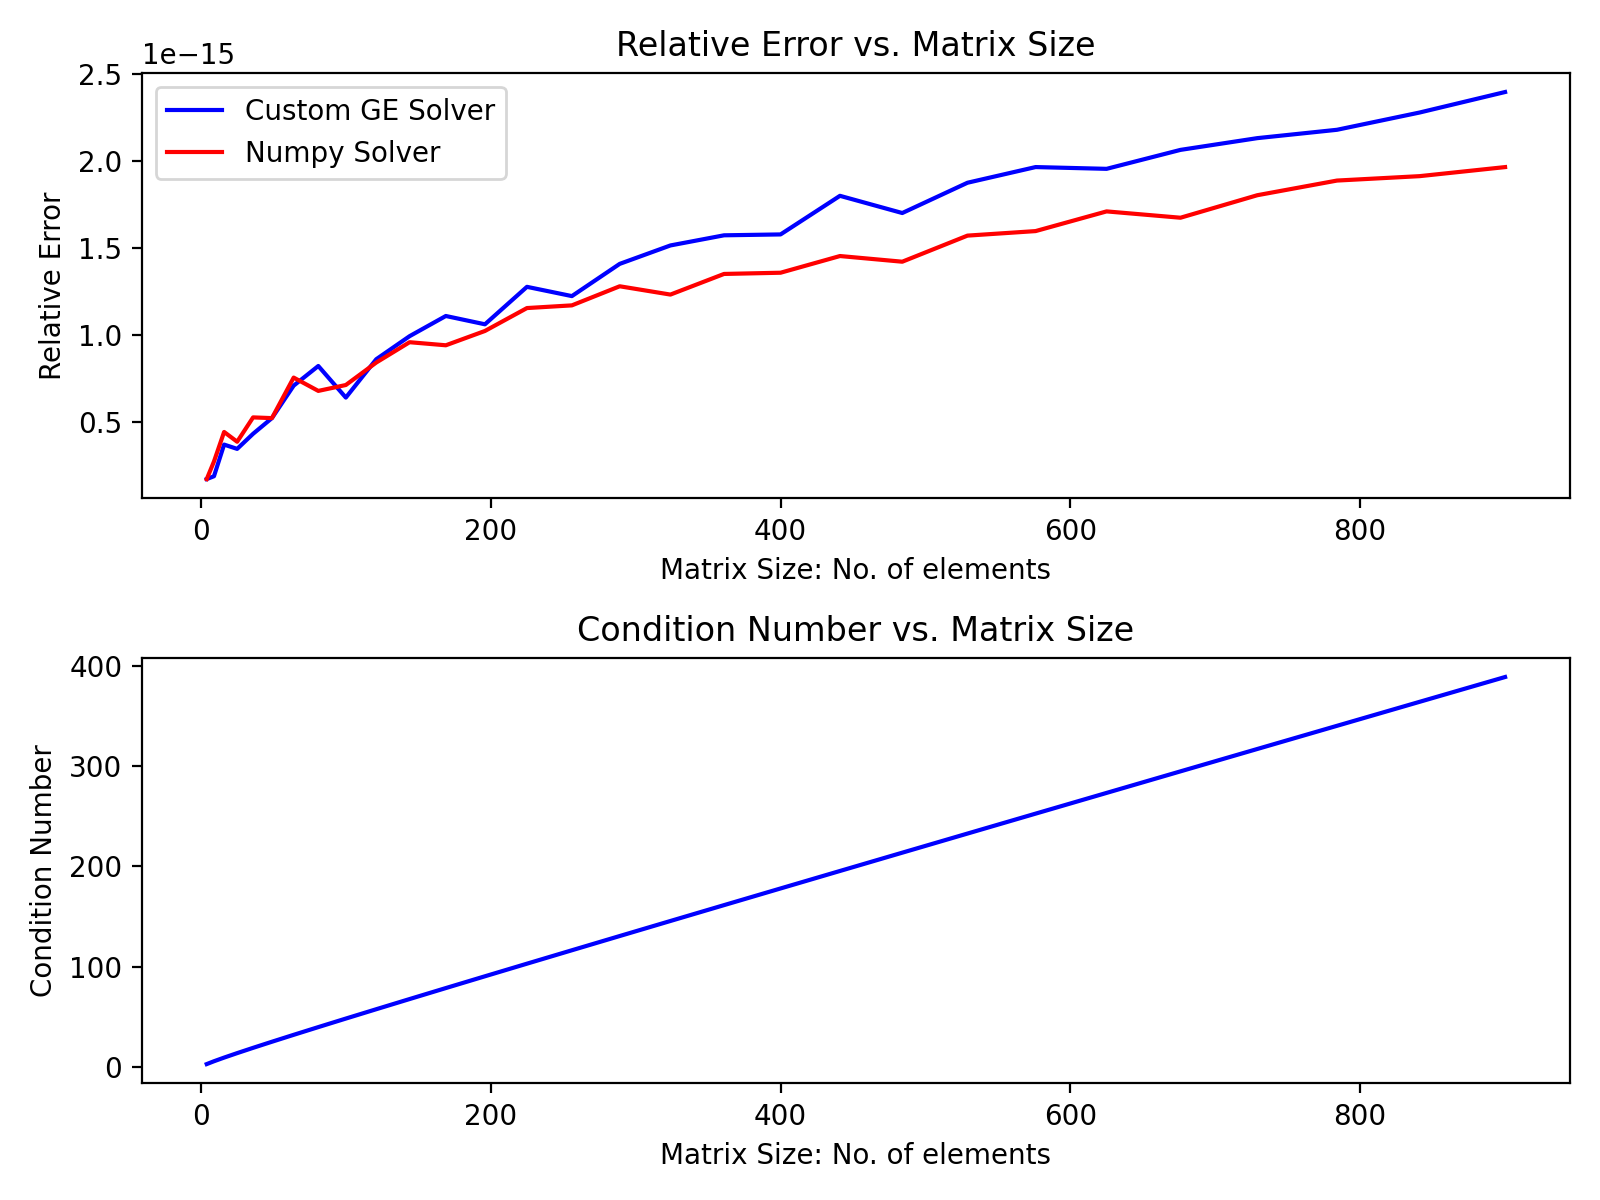
\includegraphics[width=0.9\linewidth]{rel_errs}
		\caption[Relative Errors]{Relative Error of the solution (Top) and Condition Number  of the A-Matrix (Bottom) as a function of the number of matrix elements. The relative error likely scales with the square root of the number of matrix elements (i.e. with $n$), while the condition number scales linearly with the number of matrix elements (i.e., with $n \times n$.)}
		\label{fig:relerrs}
	\end{figure}
	To answer Problem 2 - 4, we solved the same problem for various matrix sizes, from $n=2$ to $n=31$. Because the custom Gauss-Elimination solution has $\mathcal{O}(n^3)$ time complexity, we did not exceed $n=31$, because the solve time increased precipitously. The relationship between relative error and number of matrix elements appears to follow a square-root relationship: the relative error scales linearly with the number of equations being solved, $n$.
	Meanwhile, the condition number of the A matrix scales with the number of elements in the matrix.
	To verify our solver, we can build a heatmap of temperatures. First, we verify our solver by checking its solution against the example problem in \cite[p. 871]{chapraNumericalMethodsEngineers2020}. This is shown in \cref{fig:heatmap3x3}.
	\begin{figure}
		\centering
		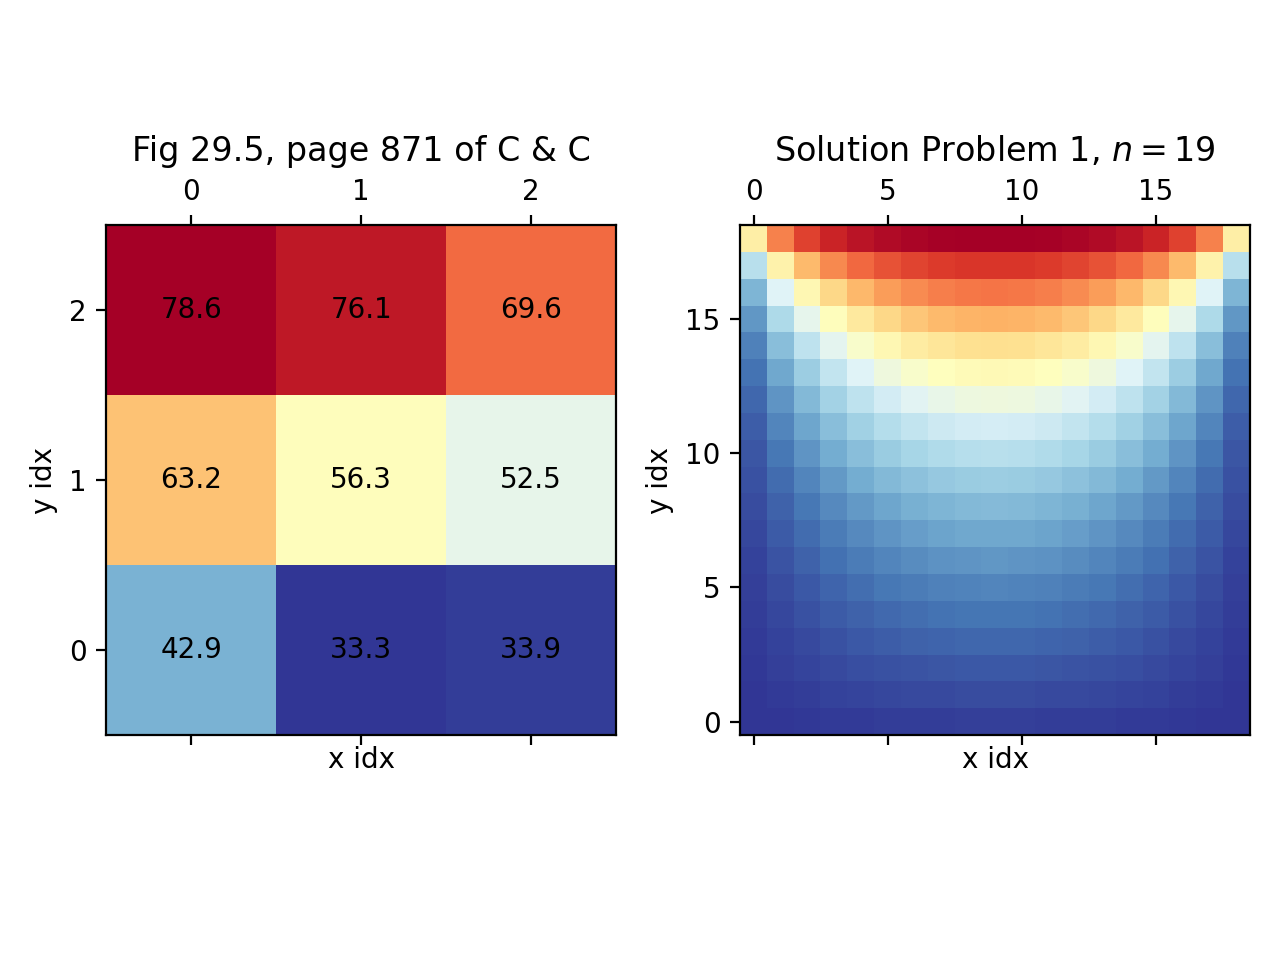
\includegraphics[width=0.9\linewidth]{heateqn.png}
		\caption[Heatmap]{Left: Heatmap of the solution to the problem in \cite[p. 871]{chapraNumericalMethodsEngineers2020}. Right: Heatmap of the solution to problem 2 for $n=19$.}
		\label{fig:heatmap3x3}
	\end{figure}
	Our solution scales well for larger cell counts, as we can see in \cref{fig:heatmap31x31} -- except runtime, of course: solving for the $31\times31$ matrix takes about 3 minutes for a 2015 MacBook Pro.
	\begin{figure}
		\centering
		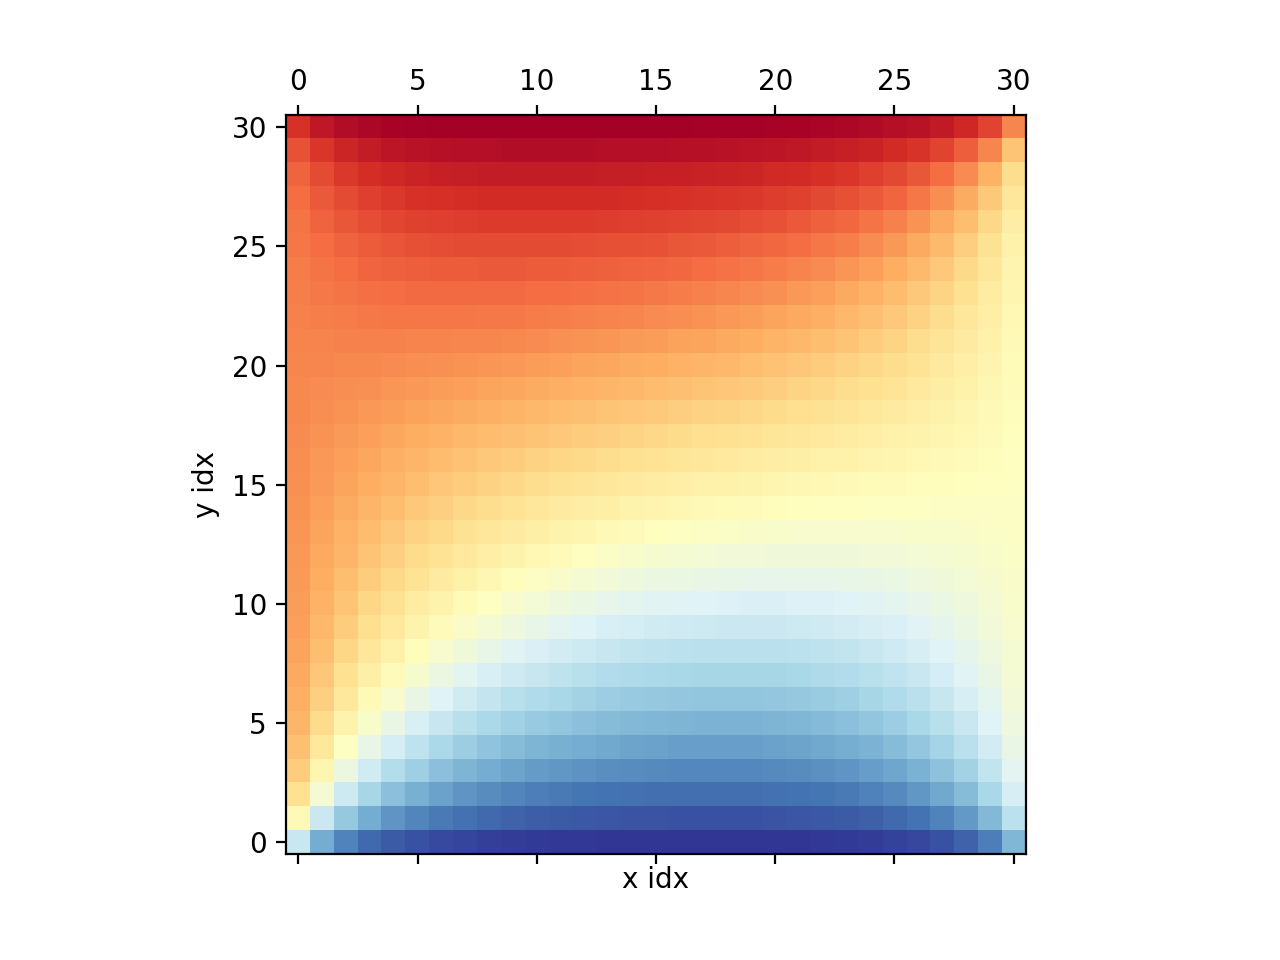
\includegraphics[width=0.6\linewidth]{heateqn_31x31.png}
		\caption[Heatmap]{Heatmap of the solution to the problem in \cite[p. 871]{chapraNumericalMethodsEngineers2020}, but scaled to $n=31$.}
		\label{fig:heatmap31x31}
	\end{figure}
	\subsection{Runtime}
	As we expect from a Gauss Elimination solver, runtime is $\mathcal{O}(n^3)$, where $n$ is the number of matrix elements. This naive implementation is not particularly efficient. We can improve performance by exploiting the fact that the matrix is diagonally dominant and sparse, which would allow us to use an $\mathcal{O}(n^2)$ algorithm like Gauss-Seidel to find the solution.
	In \cref{fig:complexity}, we look at the solution time for our algorithm, vs. the solution time for the equivalent \texttt{numpy.linalg.solve} routine for the same matrix.
	\begin{figure}
		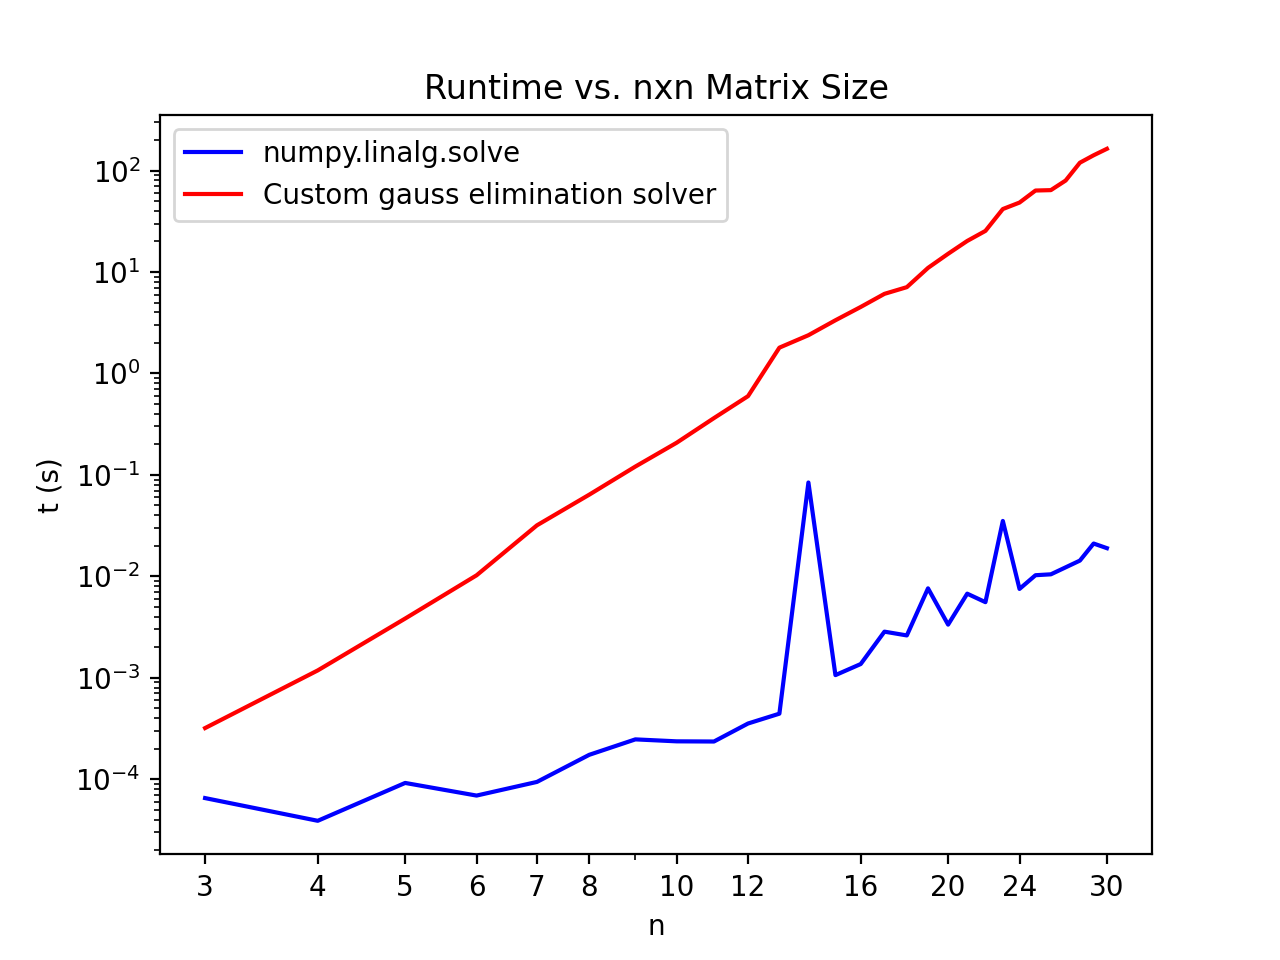
\includegraphics[width=0.9\linewidth]{runtime_vs_n.png}
		\caption[Runtime vs. Matrix Size]{Runtime of the solver (y-axis) vs. the $n$ of $n\times n$ matrix (x-axis). Both axes are log scale, which clearly shows the $\mathcal{O}(n^3)$ of the Gauss Elimination solver.}
		\label{fig:complexity}
	\end{figure}
	With some digging \cite{ali_mAnswerWhyDoes2015}, we discover that numpy uses the LAPACK solver, which is written in FORTRAN 77. Numpy uses a version of LAPACK maintained by Intel, which uses fast iterative methods on single precision, and only falls back to double precision if solutions cannot be computed. These routines are also optimized for the x86 architecture. This means that the solver is much faster than the naive implementation. \cite{Gesv}
	\section{Source Code}
	The source used to generate plots in this report, as well as the LaTeX source, can be found at \url{https://github.com/rland93/MAE195} in the "HW2" folder.
	\printbibliography
\end{document}